% --------------------------------------------------------------------------
% Template for IWAENC 2022 papers; to be used with:
%          spconfa4.sty  - ICASSP/ICIP LaTeX style file, and
%          IEEEbib.bst - IEEE bibliography style file.
%
% (Last modified by H. Loellmann, LMS, FAU Erlangen-Nuremberg, Jan. 2020)
%
% --------------------------------------------------------------------------

\documentclass{article}
\usepackage[preprint]{spconfa4}
\usepackage{amsmath,graphicx}
\usepackage[dvipsnames]{xcolor}
\usepackage{tikz}
\usetikzlibrary{arrows,snakes,backgrounds,matrix,patterns,positioning,fadings}
\usepackage{standalone}
\usepackage{subfig}
\usepackage{upgreek}
\usepackage{nicefrac}
\usepackage{dsfont}
\usepackage{bm}
\usepackage{cancel}
\usepackage{amsbsy}
\usepackage{algorithm}
\usepackage{algpseudocode}
\usepackage{lipsum}
\usepackage{harpoon}
\usepackage{comment}
\newenvironment{note}
 {\par\textcolor{Blue}{\bfseries Note:} \color{Blue}\ignorespaces}
 {\par}
\newenvironment{attention}
 {\par\textcolor{red}{\bfseries Attention:} \color{red}\ignorespaces}
 {\par}
\usepackage{hyperref}
\hypersetup{
	colorlinks,
	linkcolor={blue!80!black},
	citecolor={blue!80!black},
	urlcolor={blue!80!black}
}

\newcommand{\mtxb}[1]{\bm{\mathrm{#1}}}
\newcommand{\T}{{\mathrm{T}}}
\newcommand{\herm}{{\mathrm{H}}}
\newcommand{\ev}[1]{\mathrm{E} \left\lbrace #1 \right\rbrace}
\ninept

% \excludecomment{note}
% \excludecomment{attention}

% Common variables
\newcommand{\h}{\mtxb{h}}
\newcommand{\x}{\mtxb{x}}
\newcommand{\R}{\mtxb{R}}
\newcommand{\w}{\mtxb{w}}
\newcommand{\z}{\mtxb{z}}
\newcommand{\uu}{\mtxb{u}}
\newcommand{\aRho}{\mtxb{P}}
\newcommand{\hf}{{\bm{h}}}
\newcommand{\xf}{{\bm{x}}}
\newcommand{\Rf}{{\bm{{R}}}}
\newcommand{\wf}{{\bm{w}}}
\newcommand{\zf}{{\bm{z}}}
\newcommand{\uuf}{{\bm{u}}}
\newcommand{\aRhof}{{\bm{{P}}}}
\newcommand{\I}{\mtxb{I}}
\newcommand{\Cset}{\mathcal{C}}
\newcommand{\Csetb}{\bar{\mathcal{C}}}
\newcommand{\Mset}{\mathcal{M}}
\newcommand{\Nset}{\mathcal{N}}



% IMPORTANT: Add copyright notice by uncommenting the appropriate line
%----------------------------------------------------------
% For papers in which all authors are employed by the US government,
% \copyrightnotice{U.S. Government work not protected by U.S. copyright}

% For papers in which all authors are employed by a Crown government (UK, Canada, and Australia)
% \copyrightnotice{978-1-6654-6867-1/22/\$31.00~\copyright2022 Crown}

% For papers in which all authors are employed by the European Union,
% \copyrightnotice{978-1-6654-6867-1/22/\$31.00~\copyright2022 European Union}

% For all other papers the copyright notice is
\copyrightnotice{978-1-6654-6867-1/22/\$31.00~\copyright2022 IEEE}

% Title.
% ------
\title{DISTRIBUTED CROSS-RELATION-BASED FREQUENCY-DOMAIN\\ BLIND SYSTEM IDENTIFICATION USING ONLINE-ADMM}
%
% Single address.
% ---------------
\name{M. Blochberger\sthanks{This research work was carried out at the ESAT Laboratory of KU Leuven, in the frame of the SOUNDS European Training Network. This project has received funding from the European Union's Horizon 2020 research and innovation programme under the Marie Skłodowska-Curie grant agreement No. 956369. Source code available at \url{https://github.com/SOUNDS-RESEARCH/iwaenc2022-admm-bsi}.}, F. Elvander\sthanks{This work was supported in part by the Research Foundation - Flanders (FWO) grant 12ZD622N.}, R. Ali, T. van Waterschoot, M. Moonen, J. Østergaard, J. Jensen}
\address{KU Leuven\\Department of Electrical Engineering (ESAT)\\STADIUS Center for Dynamical Systems, Signal Processing and Data Analytics \\3001 Leuven, Belgium}
%
\begin{document}
%\ninept
%
\maketitle
%
\begin{abstract}
    In this paper, we propose a distributed cross-relation-based adaptive algorithm for blind identification of single-input multiple-output (SIMO) systems in the frequency domain using the alternating direction method of multipliers (ADMM) in a sensor network with a fusion center.
    The network consists of a fixed number of nodes each equipped with a processing unit as well as a sensor that represents an output channel of the SIMO system.
    The proposed algorithm exploits the separability of the cross-channel relations by splitting the multichannel identification problem into sub-problems involving a subset of channels which is determined by the network topology.
    Each network node delivers estimates for the subset of channel frequency responses, which then are communicated to the networks fusion center and combined into a consensus estimate per channel using general form consensus ADMM in an adaptive updating scheme.
    With numerical simulations, we show that it is possible to achieve convergence speeds and estimation errors comparable to fully centralized low-cost frequency-domain algorithms and a high-performing Quasi-Newton algorithm.
\end{abstract}
%
\begin{keywords}
    blind system identification, multichannel signal processing, distributed signal processing, ADMM, Online-ADMM
\end{keywords}
%
\section{Introduction}
\label{sec:intro}


The problem of blind system identification (BSI), which aims to estimate channel impulse responses of an unknown system without knowing the input signal, has been the subject of extensive research over recent decades.
It was introduced in \cite{satoMethodSelfRecoveringEqualization1975} and various algorithms have been proposed since.
Early algorithms used higher-order statistics \cite{godardSelfRecoveringEqualizationCarrier1980,tongNewApproachBlind1991,mecidel1991tutorial} for channel estimation, however a high computational complexity has motivated research into algorithms using only second-order statistics.
Suh algorithms include the cross-relation (CR) algorithm \cite{tong1994blind, guanghanxuLeastsquaresApproachBlind1995}, subspace algorithms \cite{moulinesSubspaceMethodsBlind1995,gannotSubspaceMethodsMultimicrophone2003,diamantarasEfficientSubspaceMethod2008,mayyalaStructureBasedSubspaceMethod2017} and maximum-likelihood algorithms \cite{yingbohuaFastMaximumLikelihood1996}.
Out of various multichannel BSI algorithms which have been proposed, adaptive cross-relation-based least-mean-squares (LMS) algorithms in the time and frequency domain are the ones most widely used.
The normalized multi-channel frequency-domain LMS (NMCFLMS) \cite{huangAdaptiveMultichannelLeast2002,huangClassFrequencydomainAdaptive2003} algorithm for instance is an efficient algorithm utilizing the fast Fourier transform (FFT) which has been extended to include constraints to improve robustness to noise and performance on acoustic impulse responses (RNMCFLMS \cite{huNoiseRobustBlind2015}, \(l_p\)-RNMCFLMS \cite{heNoiseRobustFrequencyDomain2018}, phase-constrained-\(l_p\)-RNMCFLMS \cite{joRobustBlindMultichannel2021}).
The quasi-Netwon algorithm \cite{habetsOnlineQuasiNewtonAlgorithm2010} on the other hand is a time-domain algorithm that utilizes the BFGS method to estimate the Hessian of the problem.

While there exist distributed signal processing algorithms for applications such as noise cancellation \cite{}, echo control \cite{} or beamforming \cite{}, there is a gap regarding BSI which we are starting to fill with this contribution.
The general-form consensus alternating direction method of multipliers (ADMM) \cite{boydDistributedOptimizationStatistical2011} solves optimization problems with cost functions separable in its variable.
We separate the inter-channel cross-relations of the BSI problem according to the networks topology, i.e. each node 

to form smaller sub-problems involving overlapping subsets of the entire channel set and use equality constraints to find a consensus on the overlapping estimated sub-problem parameters.

% The alternating direction method of multipliers (ADMM) \cite{boydDistributedOptimizationStatistical2011} solves optimization problems by splitting them into smaller sub-problems, each less complex to solve than the original one.
% In this paper, we use ADMM to separate the inter-channel cross-relations to form smaller sub-problems involving overlapping subsets of the entire channel set and use equality constraints to find a consensus on the overlapping estimated sub-problem parameters.
% The ADMM update steps are applied in a block processing scheme forming an adaptive algorithm also referred to as Online-ADMM \cite{wangOnlineAlternatingDirection2013,hosseiniOnlineDistributedADMM2014}.

As shown in numerical simulations, the resulting algorithm provides good estimation results as compared to state-of-the-art algorithms while keeping the computational complexity low and providing scalability through distributed processing possibilities.
% All code to generate the results and this paper are available at \cite{Blochberger_CROSS-RELATION-BASED_FREQUENCY-DOMAIN_BLIND_2022}

% #############################################################################
% #############################################################################
\section{Problem statement}
\label{sec:problem_statement}


% #############################################################################
\subsection{Signal Model}
\label{ssec:signal_model}
We consider an acoustic SIMO system with the input signal \(\mtxb{s}(n)\) and \(M\) outputs \(\x_i(n)\) defined as
\begin{align}
    \mtxb{s}(n) &= \begin{bmatrix}
        s(n)&s(n-1)&\ldots&s(n-2L+2)
    \end{bmatrix}^{\T}\\
    \x_i(n) &= \begin{bmatrix}
        x_i(n)&x_i(n-1)&\ldots&x_i(n-L+1)
    \end{bmatrix}^{\T}.
\end{align}
where \(i \in \Mset \triangleq \{1,\ldots,M\} \).
Each output \(\x_i(n)\) is the convolution of \(\mtxb{s}(n)\) with the respective channel impulse response \(\h_i\) and an additive noise term \(\mtxb{v}_i(n)\), assumed to be zero-mean and uncorrelated to \(\mtxb{s}(n)\).
The signal model is described by
\begin{equation}
    \x_i(n) = \mtxb{H}_i \mtxb{s}(n) + \mtxb{v}_i(n),
\end{equation}
where \(\mtxb{H}_i\) is the \(L \times (2L-1)\) linear convolution matrix of the \(i\)th channel using the elements of \(\h_i\) of length \(L\) which represents the system to be identified.
The impulse response length \(L\) is assumed to be known.

% #############################################################################
\subsection{Cross-relation approach}
\label{ssec:cross_rel}
The cross-relation approach for BSI aims to use only the output signals of the system to identify it.
This can be achieved by exploiting the relative channel information when more than one channel is available, and the identifiability conditions \cite{guanghanxuLeastsquaresApproachBlind1995} are satisfied. These conditions are: (i) the channel transfer functions have no common zeros (i.e. are not co-prime), and (ii) the covariance matrix of the input signal \(\mtxb{s}(n)\) is of full rank (i.e. the signal has a number of modes \(\geq 2L+1\)).

The fundamental equality of this approach in the noiseless case \(\mtxb{v}_i(n) = 0\), is 
\begin{equation}
    \x_i^{\T}(n) \h_j = \x_j^{\T}(n) \h_i,\quad i,j \in \Mset,\,i\neq j\label{eq:cross_rel:equality_conv}
\end{equation}
which states that the channel output signal convolved with the impulse response of another is equal to the vice-versa as follows from the commutativity property of the convolution.
Left-multiplication and applying the expectation operator to form the covariance matrix \(\R_{ij}(n) = \ev{\x_i(n) \x_j^\T(n)}\) and combining all cross-relations \eqref{eq:cross_rel:equality_conv} (see e.g. \cite{huangAdaptiveMultichannelLeast2002} for a more thourough derivation) yields the system of equations  
\begin{equation}
    \R(n) \h = \bm{0} \label{eq:cross_rel:null_space}\\
\end{equation}
where \(\R\) is an \(M L \times M L\) matrix given by:
\begin{equation}
    \R = \begin{bmatrix}
        \sum_{i \neq 1} \R_{ii} & -\R_{21} & \cdots & -\R_{M1}\\
        -\R_{12} & \sum_{i \neq 2} \R_{ii} & \cdots & -\R_{M2}\\
        \vdots & \vdots & \ddots & \vdots\\
        -\R_{1M} & -\R_{2M} & \cdots & \sum_{i \neq M} \R_{ii}\\
    \end{bmatrix}\label{eq:cross_rel:data_matrix}
\end{equation}
and \(\h = \begin{bmatrix}
    \h_1^\T & \cdots & \h_M^\T
\end{bmatrix}^\T\).
Formulating the problem in the frequency domain, the derivation is analogous. We denote all frequency-domain variables in bold cursive (e.g. \(\Rf\)) compared to the time-domain bold upright (e.g \(\R\)). The derivation involves the frame-based overlap-save technique, working with signal frames \(\x_{i,2L}(m)\) of length \(2L\), frame index \(m\), leading to the system of equations 
\begin{equation}
    \Rf(m) \hf = \bm{0} \label{eq:frequency_domain:null_space}\\
\end{equation}
where the \(M L \times M L\) matrix is recursivly estimated by \begin{equation}
    \hat{\Rf}(m) = \eta \hat{\Rf}(m-1) + (1-\eta )\tilde{\Rf}(m).
\end{equation}
where \(\eta \in [0,1]\) is an exponential smoothing factor and \(\tilde{\Rf}(m)\) is constructed analogous to \eqref{eq:cross_rel:data_matrix}, however with covariance matrices replaced by instantaneous cross-spectrum matrices 
\begin{equation}
    \tilde{\Rf}_{ij}(m) = \bm{X}_{i} (m) \bm{X}_{j}^\herm (m)
\end{equation}
with 
\begin{equation}
    \bm{X}_{i}(m) = \bm{{W}}^{01}_{L \times 2L} \bm{{D}}_{i}(m) \bm{{W}}^{10}_{2L \times L}.
\end{equation}
The matrix \(\bm{{D}}_{i}(m) = \operatorname{diag} \left\{ \operatorname{FFT}_{2L} \left\{ \x_{i,2L}(m) \right\} \right\}\) contains the  signal spectrum on its diagonal and
\begin{align}
    \bm{{W}}_{L \times 2L}^{01} &= \mtxb{F}_{L \times L} \mtxb{W}_{L \times 2L}^{01} \mtxb{F}_{2L \times 2L}^{-1}\\
    \bm{{W}}_{2L \times L}^{10} &= \mtxb{F}_{2L \times 2L} \mtxb{W}_{2L \times L}^{10} \mtxb{F}_{L \times L}^{-1}
\end{align} are the frequency-domain overlap-save matrices where \(\mtxb{F}_{L \times L}\) and \(\mtxb{F}_{2L \times 2L}\) are the discrete Fourier transform (DFT) matrices for sizes L and 2L respectively and \(
    \mtxb{W}_{L \times 2L}^{01} = \begin{bmatrix}
        \mtxb{0}_{L \times L} & \mtxb{I}_{L \times L}
    \end{bmatrix}\)
    and \(
    \mtxb{W}_{2L \times L}^{10} = \begin{bmatrix}
        \mtxb{I}_{L \times L} & \mtxb{0}_{L \times L}
    \end{bmatrix}^\T\)
denote the time-domain overlap-save matrices.

Analogous to the time-domain formulation, the vector \(\hf\) is a stacked vector of complex-valued frequency responses.
In the presence of noise, the system of equations \eqref{eq:frequency_domain:null_space} is best solved by posing it as a least-mean-squares minimization problem \cite{guanghanxuLeastsquaresApproachBlind1995,huangAdaptiveMultichannelLeast2002}:
%  minimizing \(\|\underline{\bm{e}} \|^2 = \| \Rf \hf \|^2\) with the constraint \(\hf^\herm \hf = a\) to avoid the trivial zero solution.
% As this effectively seeks the \(a\)-scaled eigenvector of the squared hermitian matrix \(\Rf^\herm \Rf\) corresponding to the smallest eigenvalue, we can replace it with its non-squared form \(\Rf\) as the eigenvectors for both are equal.
% To compute the estimates, we minimize the cost function
% \begin{equation}
%     J(\hf)(m+1) = \hf^\herm(m) \Rf(m) \hf(m)\label{eq:frequency_domain:cost_function}
% \end{equation}
% as the minimization problem
\begin{align}
    \hat{\hf} = \arg \min_{\hf} \quad &\hf^\herm \hat{\Rf} \hf \label{eq:frequency_domain:min_prob}\\
    \text{s.t. } \quad &\hf^\herm \hf = 1.
\end{align}

In the following section, we introduce an adaptive algorithm using ADMM to find a solution to this problem.

% #############################################################################
% #############################################################################
\section{Proposed Algorithm}
\label{sec:proposed_method}

% #############################################################################
\subsection{Problem Splitting}
\label{ssec:problem_splitting}
In state-of-the-art algorithms \cite{heNoiseRobustFrequencyDomain2018,habetsOnlineQuasiNewtonAlgorithm2010}, the minimization problem \eqref{eq:frequency_domain:min_prob} is solved in its full form resulting in potentially high computational effort when the number of channels and length of impulse responses or number of DFT bins is large.
Here however, we split the problem into \(N \in \mathbb{N}\) sub-problems and denote the index set of these \(N\) sub-problems as \(\Nset \triangleq \{1,\ldots,N\}\).
Each sub-problem is defined by a subset of the full channel set \(\Cset_i \subseteq \Mset\) with \(i \in \Nset\).
Following from that, we define the sets \(\Csetb_j = \left\{ i \vert j \in \Cset_i \right\}\) for \(i,j \in \Mset\) where for each channel \(j\) a set represents the sub-problems that particular channel is part of.
% This channel-to-sub-problem relation can also be represented as a \(M \times N\) matrix \(\mtxb{G}\) where the sets \(\Cset_i\) and \(\Csetb_j\) are the indices of non-zero elements of the rows and columns respectively (see \autoref{fig:problem_splitting:problem_splitting_matrix}).
Further, \(M_i = \left| \Cset_i \right| \) and \(N_j = \left| \Csetb_j \right| \) with \(i,j \in \Mset\).

We replace the cost function minimized in \eqref{eq:frequency_domain:min_prob} with the separable cost function 
\begin{equation}
    \tilde{J}(\hf) = \sum_{i \in \Nset} \tilde{J}_i(\wf_i)  = \sum_{i \in \Nset} \wf_i^\herm \hat{\aRhof}_i \wf_i
    \label{eq:problem_splitting:cost_function}
\end{equation}
where \(\wf_i\) is defined as the stacked vector of estimated frequency responses analogous to \(\hf\) (cf. \autoref{ssec:cross_rel}) and \(\hat{\aRhof}\) is constructed as defined in \eqref{eq:cross_rel:data_matrix}, both using the respective subset \(\Cset_i\).
If the channel subsets are proper \(\Cset_i \subset \Mset\), this leads to \(N\) sub-problems, each with smaller dimensions than the original centralized problem, reducing complexity.
The lowest-dimensionality is attained when each \(\Cset_i\) has two elements, i.e. two channels, assuming perfect parallel processing, effectively reducing problem size from \(ML \times ML\) to \(2L \times 2L\).

% \begin{figure}
%     \centering
%     \subfloat[][]{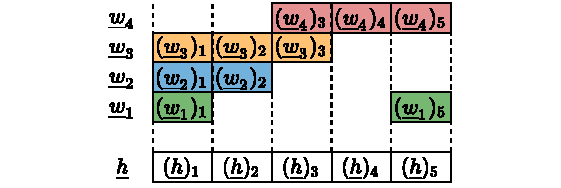
\includegraphics[trim={1.8cm 0 1.7cm 0},clip,scale=0.7]{images/parameter_mapping.pdf}}
%     \subfloat[][]{\includestandalone[trim={0.65cm 0 0 0},clip,scale=0.7]{tikz/connection_matrix}}
%     \subfloat[][]{\includestandalone[trim={0.6cm 0 0 0},clip,scale=0.6]{tikz/problem_splitting_matrix}}
%     % \includestandalone[scale=1]{tikz/topology_general}
%     \vspace*{-0.3cm}
%     \caption{Problem splitting and parameter mapping for a general case with \(M=5\) channels and \(N=4\) sub-problems. (a) shows the mapping of the local estimate components \((\wf_i)_j\) to the global consensus components \((\hf)_j\) via \(\mathcal{G}(i,j)\), (b) \(\mtxb{G}\) with 1 (\(\blacksquare\)) and 0 (\(\square\)), (c) shows \(i,j\)-cross-relations used by sub-problems compared to full \(M\)-channel problem.}
%     \label{fig:problem_splitting:problem_splitting_matrix}
% \end{figure}

\begin{figure}
    \centering
    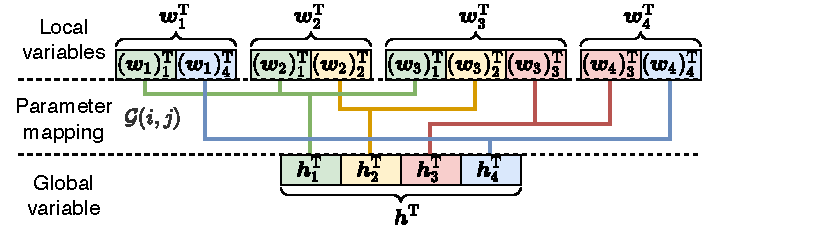
\includegraphics[trim={0.3cm 0.25cm 1.7cm 0.0cm},clip,width=\columnwidth]{images/parameter_mapping2.pdf}
    % \includestandalone[scale=1]{tikz/topology_general}
    \vspace*{-0.5cm}
    \caption{Parameter mapping of the local variable components \(({\wf}_i)_j\) to the global consensus variable components \(({\hf})_j\) via \(\mathcal{G}(i,j)\) for a general case with \(M=4\) channels and \(N=4\) sub-problems.}
    \label{fig:problem_splitting:problem_splitting_matrix}
\end{figure}

% #############################################################################
\subsection{General-Form Consensus ADMM}
\label{ssec:general_consensus_admm}
Minimization problems with separable cost functions can be solved by the well-established method of consensus ADMM \cite{boydDistributedOptimizationStatistical2011}.
In the previous section we introduced the split cost function \eqref{eq:problem_splitting:cost_function} which we now set in the context of the general-form consensus problem
\begin{align}
    \operatorname{minimize} \quad &\sum_{i \in \Nset} \tilde{J}_i(\wf_i)\\
    \text{subject to} \quad &(\wf_i)_j = \hf_{\mathcal{G}(i,j)},\quad i \in \Nset,\,j \in \Cset_i
\end{align}
where \(\mathcal{G}(i,j)\) denotes the mapping of \(L\) local variable components \((\wf_i)_j\), i.e. one of the frequency responses in the stacked vector, to the corresponding global variable components \((\hf)_g\) (cf. \autoref{fig:problem_splitting:problem_splitting_matrix}).
For brevity, the mapped global variables \((\tilde{\hf}_i)_j = \hf_{\mathcal{G}(i,j)}\) are introduced.
The equality constraint between local variables \(\wf_i\) and global variable \(\hf\) enforces the consensus, i.e. a common solution taking into account data of all sub-problems.

The augmented Lagrangian for this particular general-form consensus problem is
\begin{align}
    \mathcal{L}_{\rho} (\wf,\hf,\uuf) &= \sum_{i \in \Nset} \left( \wf_i^\herm \hat{\aRhof}_i \wf_i + 2 \Re \left( \uuf_i^{\herm} \left(\wf_i - \tilde{\hf}_i\right) \right)\right. \vphantom{+ \rho \left\| \wf_i - \tilde{\hf}_i \right\|} \nonumber\\
    \vphantom{\wf_i^\herm \hat{\aRhof}_i \wf_i + 2 \Re \left( \uuf_i^{\herm} \left(\wf_i - \tilde{\hf}_i\right) \right)} & \qquad \qquad \qquad \qquad \left.+ \rho \left\| \wf_i - \tilde{\hf}_i \right\|^2 \right)\label{eq:general_consensus_admm:lagrangian}
\end{align}
% \begin{align}
%     &\mathcal{L}_{\rho} (\wf,\hf,\uuf) = \sum_{i \in \Nset} \left( \wf_i^\herm \hat{\aRhof}_i \wf_i + \uuf_i^{\herm} \left(\wf_i - \tilde{\hf}_i\right)\vphantom{+ \frac{\rho}{2} \left\| \wf_i - \tilde{\hf}_i \right\|^2} \right.\nonumber\\
%     &\left. + \left(\wf_i - \tilde{\hf}_i\right)^\herm \uuf_i + \left( \wf_i - \tilde{\hf}_i \right)^\herm \rho \I \left( \wf_i - \tilde{\hf}_i \right) \right).\label{eq:general_consensus_admm:lagrangian}
% \end{align}
The ADMM then consists of the steps:
\begin{align}
    \wf_i^{k+1} &= \underset{\wf_i}{\operatorname{argmin}} \, \mathcal{L}_{\rho} (\wf,\hf^k,\uuf^k),\label{eq:general_consensus_admm:local}\\
    \hf^{k+1} &= \underset{\hf, \|\hf\| = 1}{\operatorname{argmin}}\, \mathcal{L}_{\rho} (\wf^{k+1},\hf,\uuf^k)\label{eq:general_consensus_admm:global}\\
    \uuf_i^{k+1} &= \uuf_i^{k} + \rho \left( \wf_i^{k+1} - \tilde{\hf}_i^{k+1} \right).\label{eq:general_consensus_admm:dual}
\end{align}
% \begin{align}
%     &\wf_i^{k+1} = \underset{\wf_i}{\operatorname{argmin}} \left\{ \wf_i^\herm \hat{\aRhof}_i \wf_i + \uuf_i^{k\,\herm} \left(\wf_i - \tilde{\hf}_i^{k}\right) \vphantom{+ \left\| \wf_i - \tilde{\hf}_i^{k} \right\|^2}\right.\nonumber\\
%     &\left.+ \left(\wf_i - \tilde{\hf}_i^{k}\right)^\herm \uuf_i^{k} + \left( \wf_i - \tilde{\hf}_i^{k} \right)^\herm \rho \I \left( \wf_i - \tilde{\hf}_i^{k} \right) \right\},\label{eq:general_consensus_admm:local}\\
%     &\hf^{k+1} = \underset{\hf, \|\hf\| = a}{\operatorname{argmin}} \left\{ \sum_{i \in \Mset} \left( \tilde{\hf}_i^{\herm} \uuf_i^{k} + \uuf_i^{k\,\herm} \tilde{\hf}_i \vphantom{\frac{\rho}{2} \| \wf_i^{k+1} - \tilde{\hf}_i \|^2} \right.\right.\nonumber\\
%     &\left. \qquad \qquad \vphantom{\sum_{i=1}^{M} pp } \left.+ \left( \wf_i^{k+1} - \tilde{\hf}_i \right)^\herm \rho \I \left( \wf_i^{k+1} - \tilde{\hf}_i \right)  \right) \right\},\label{eq:general_consensus_admm:global}\\
%     &\uuf_i^{k+1} = \uuf_i^{k} + \rho \left( \wf_i^{k+1} - \tilde{\hf}_i^{k+1} \right).\label{eq:general_consensus_admm:dual}
% \end{align}
As this is still denoted as an iterative algorithm, we will introduce the online/adaptive aspect of the proposed algorithm in the following.

\subsection{Online ADMM-BSI}
\label{ssec:online_admm}
We introduced the original problem in \eqref{eq:frequency_domain:null_space} with time-dependent data matrix. It therefore follows that the data term in \eqref{eq:general_consensus_admm:lagrangian} is also time-dependent, which from here on will be denoted with the additional superscript time index \(m\) as \(\wf_i^\herm \hat{\aRhof}_i^{m} \wf_i\).
A thorough overview of time-varying data terms in ADMM can be found in \cite{wangOnlineAlternatingDirection2013,hosseiniOnlineDistributedADMM2014} where it is referred to as ``Online-ADMM".

We transform the iterative batch processing method \eqref{eq:general_consensus_admm:local}-\eqref{eq:general_consensus_admm:dual} into an adaptive one by computing only a (small) finite number of iterations with each time-frame-\(m\) specific data term.
Here specifically, we apply one iteration per time frame, which manifests itself as simply replacing the iteration index \(k\) with the time index \(m\)

The minimization problem for the local variable \(\wf_i\) \eqref{eq:general_consensus_admm:local} can be solved by various algorithms, in this case however we perform the update step
\begin{equation}
    \wf_i^{m+1} = \wf_i^{m} - \mu \bm{{V}}_i^m \left( \hat{\aRhof}_i^m \wf_i^m + \uuf_i^m + \rho\left(\wf_i^m - \tilde{\hf}_i^{m}\right)\right)\label{eq:online_admm:local_update}
\end{equation}
where \(\mu\) (\(0  < \mu\leq 1\)) is a step size and \(\bm{{V}}_i^m = \left(\hat{\aRhof}_i^m + \rho \I \right)^{-1}\) is the inverse Hessian of the problem.
As this inverse is costly to compute, it is approximated by a diagonalized matrix
\begin{equation}
    \tilde{\bm{{V}}}_i^m = \operatorname{diag} \left\{ \left( \operatorname{diag} \left\{ \hat{\aRhof}_i^m \right\} + \rho \mtxb{1} \right)^{-1}\right\},
\end{equation}
similar to NMCFLMS \cite{huangClassFrequencydomainAdaptive2003}, which is straightforward to compute.

For the update step of the consensus variable \(\hf\), it may be readily verified (cf. \cite{boydDistributedOptimizationStatistical2011}) that the solution to \eqref{eq:general_consensus_admm:global} is given by
\begin{equation}
    \hf^{m+1} = \frac{\bar{\wf}^{m+1} + \frac{1}{\rho} \bar{\uuf}^{m} }{\left\| \bar{\wf}^{m+1} + \frac{1}{\rho} \bar{\uuf}^{m} \right\|}.\label{eq:online_admm:consensus_update}
\end{equation}
where the \(M L \times 1\) vectors \(\bar{\wf}^{m+1}, \bar{\uuf}^{m+1}\) are computed as the mapped averages
\begin{equation}
    (\bar{\wf}^{m+1})_g = \frac{1}{N_g} \sum_{\mathcal{G}(i,j)=g} (\wf_i^{m+1})_j,\quad g,i,j \in \Mset,
\end{equation}
and
\begin{equation}
    (\bar{\uuf}^{m})_g = \frac{1}{N_g} \sum_{\mathcal{G}(i,j)=g} (\uuf_i^{m})_j,\quad g,i,j \in \Mset.
\end{equation}
This results in a computationally inexpensive update step forcing the norm of the consensus to have unit value.

% #############################################################################
% #############################################################################
\section{Numerical Evaluation}
\label{sec:perf_eval}

\begin{figure}[t]
    \centering
    \subfloat[][]{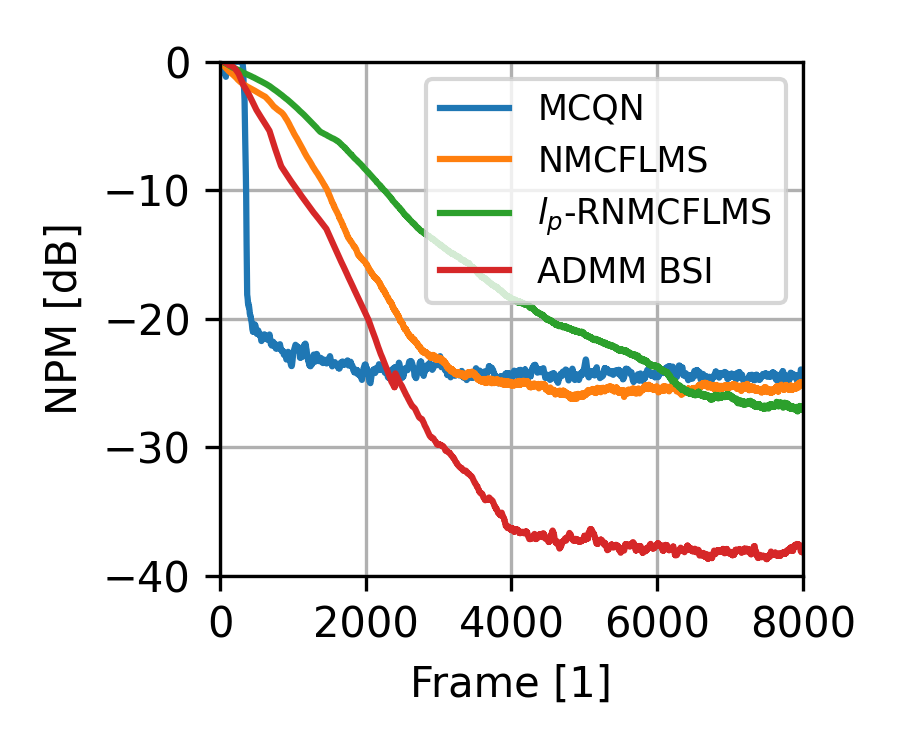
\includegraphics[trim={0.3cm 0.35cm 0.3cm 0.3cm},clip,height=4cm]{python/plots/NPM_over_time_SNR10.png}\label{fig:perf_eval:NPM_over_time_SNR10}}\\
    \vspace*{-0.3cm}
    \subfloat[][]{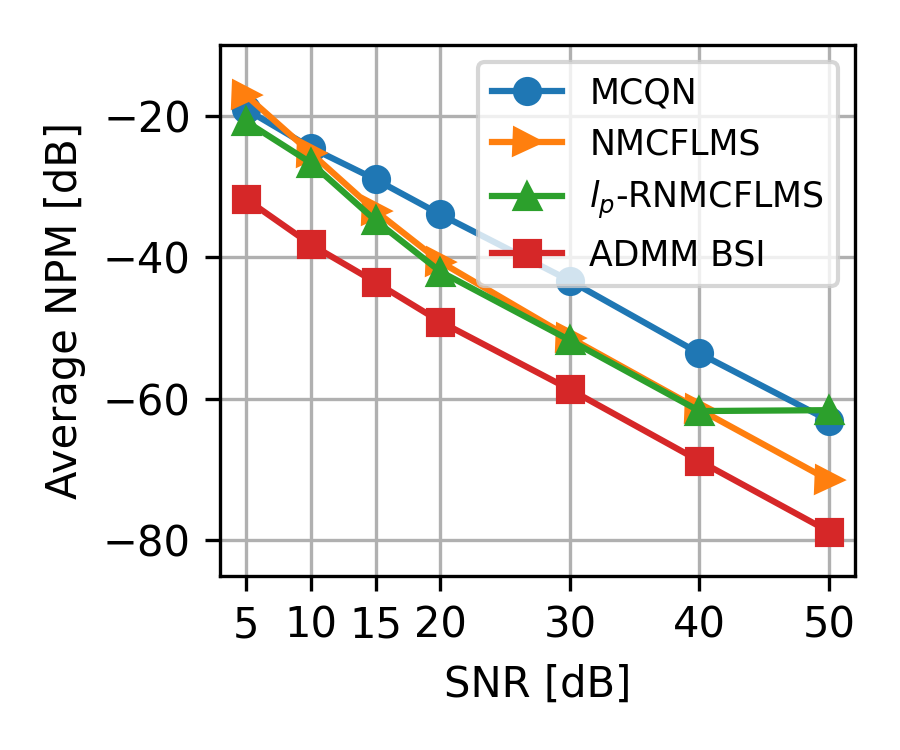
\includegraphics[trim={0.3cm 0.35cm 0.3cm 0.3cm},clip,height=4cm]{python/plots/NPM_over_SNR_L64_M5.png}\label{fig:perf_eval:NPM_over_SNR_L64_M5}}
    \vspace*{-0.2cm}
    \caption{Comparison of ADMM-BSI convergence behaviour with \(L\!=\!64\) at different SNR values. Shown are (a) NPM at \(\text{SNR}=10\,\text{dB}\) over frame index \(m\) for convergence speed comparison and (b) the steady-state NPMs over different SNRs.}
    \label{fig:perf_eval:NPM_over_time_exp1}
\end{figure}

The performance of the proposed algorithm is assessed via numerical simulations.
As an error measure, we use the normalized projection misalignment (NPM) \cite{huangClassFrequencydomainAdaptive2003}
\begin{equation}
    \text{NPM}(m) = 20\,\log_{10} \left(\frac{\left\| \h(m) - \frac{\h^\T (m) \h_{\text{t}}}{\h_{\text{t}}^\T \h_{\text{t}}}\h(m) \right\|_2}{\left\|\h(m)\right\|_2} \right)
\end{equation}
where \(\h\) is the stacked vector of impulse response estimates (cf. \autoref{ssec:cross_rel}), which are the inversely Fourier-transformed estimated frequency responses stacked in \(\hf\) and \(\h_{\text{t}}\) is the ground truth. The signal-to-noise ratio (SNR) for the simulations is defined as 
\begin{equation}
    \text{SNR} = 10 \log_{10} \left(\frac{\sigma_s^2 \| \h_t \|}{M \sigma_v^2} \right)
\end{equation}
where \(\sigma_s^2\) and \(\sigma_v^2\) are the variance of signal and noise respectively which both are modelled by (channel-independent) white Gaussian noise (WGN).

The first simulation evaluates the performance using randomly generated impulse responses of length \(L=64\) under different signal-to-noise ratios (SNR) on a 5-channel system (\(M=5,\, N=5\)).
The impulse responses are drawn from a Normal distribution with unit variance, and the signal is \(8 \times 10^{5}\) samples of WGN to ensure convergence of all algorithms.
The step sizes are hand tuned for similar convergence speed: \(\mu_{\text{MCQN}}=0.5,\, \mu_{\text{NMCFLMS}}=0.4,\, \mu_{l_p-\text{NMCFLMS}}=0.3,\, \mu_{\text{ADMM}}=0.6,\, \rho=1,\,\eta=0.98 \).
\autoref{fig:perf_eval:NPM_over_time_exp1} shows the median of 30 Monte-Carlo runs where the averaged NPM of the last \(100\) frames is plotted.
It is observable that the proposed algorithm yields a lower steady-state NPM than the compared NMCFLMS, RNMCFLMS, and \(l_p\)-RNMCFLMS algorithms.

\begin{figure}[t]
    \centering
    \hspace*{-0.2cm}\subfloat[][\(M\!=\!4,P\!=\!4\)]{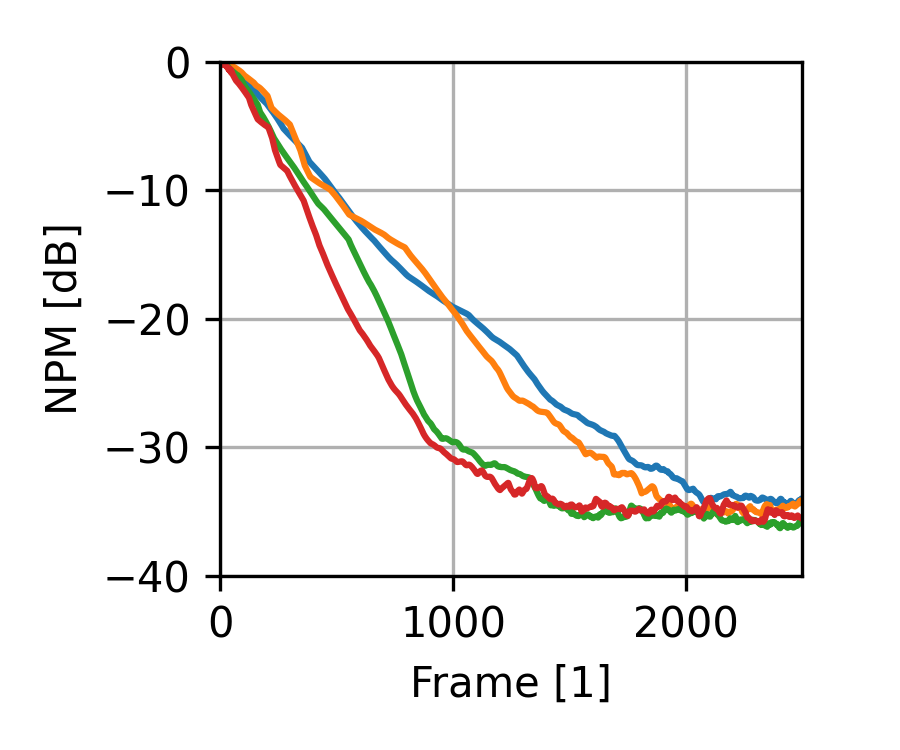
\includegraphics[trim={0.3cm 0.35cm 0.3cm 0.3cm},clip,height=3.7cm]{python/plots/NPM_over_time_M4.png}\label{fig:perf_eval:NPM_over_time_M4}}
    % \hspace*{-0.2cm}\subfloat[][\(M\!=\!4,N\!=\!4\)]{\begin{overpic}[trim={0.3cm 0.35cm 0.3cm 0.3cm},clip,height=3.7cm]{python/plots/NPM_over_time_M4.png}
    %     \put(54,48){\includestandalone[trim={0.0cm 0.0cm 0.0cm 0},clip,scale=0.5]{tikz/connection_matrix_eval}}
    % \end{overpic}\label{fig:perf_eval:NPM_over_time_M4}}
    \hspace*{-0.0cm}\subfloat[][\(M\!=\!8,N\!=\!8\)]{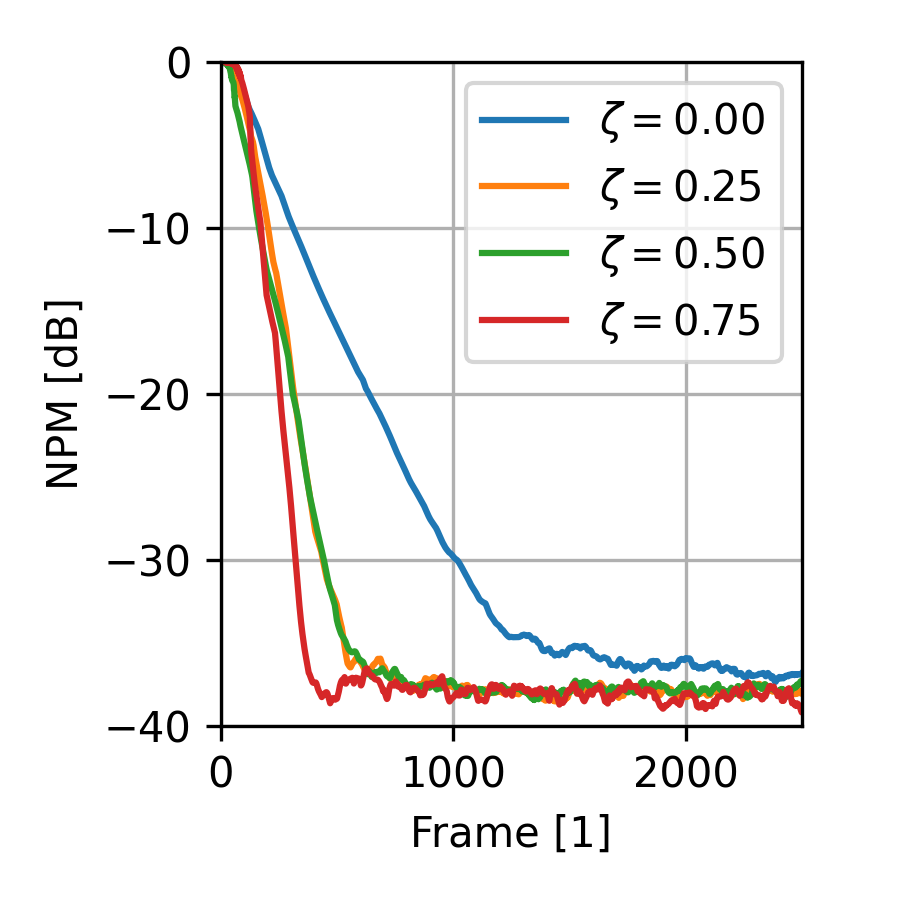
\includegraphics[trim={0.3cm 0.35cm 0.3cm 0.3cm},clip,height=3.7cm]{python/plots/NPM_over_time_M8.png}\label{fig:perf_eval:NPM_over_time_M8}}
    \vspace*{-0.2cm}
    \caption{Comparison of ADMM-BSI convergence behaviour with \(L\!=\!16\) for different values of the sub-problem overlap \(\zeta\) for \(\text{SNR}=20\,\text{dB}\).}
    \label{fig:perf_eval:NPM_over_time_exp2}
\end{figure}

The second simulation is a small-scale assessment of the influence of the overlap of sub-problems.
Two base scenarios, \(M=4,\,N=4\) and \(M=8,\,N=8\), are evaluated using short (\(L=16\)) random impulse responses and different values for the sub-problem overlap parameter \(\zeta\) which is defined as the ratio of ones to zeros of only considering elements of \(\mtxb{G}\) that are not part of the main diagonal, superdiagonal and the first element of the last row (marked gray on the inset of \autoref{fig:perf_eval:NPM_over_time_M4}).
Random patterns satisfying this definition for \(\zeta \in \{0.0,\,0.25,\,0.5,\,0.75\}\) are generated.
\autoref{fig:perf_eval:NPM_over_time_exp2} shows the median of 30 Monte-Carlo runs for the two setups, which shows the proportional relation of convergence speed, channel number \(M\) and sub-problem overlap \(\zeta\) while the steady-state error is not dependent on \(\zeta\).




% #############################################################################
% #############################################################################
\section{Conclusions}
\label{sec:conclusion}
In this paper, an adaptive ADMM algorithm for blind system identification was developed.
The algorithm separates the BSI problem into lower-dimensional sub-problems to reduce computational complexity and allows for parallel or distributed processing while maintaining steady-state error performance and convergence speed.
Preliminary results using white Gaussian noise and randomly generated impulse responses have demonstrated improved steady-state error measures compared to state-of-the-art algorithms and that  steady-state performance is not affected by speparating the BSI problem into sub-problems while convergence speed is.

% References should be produced using the bibtex program from suitable
% BiBTeX files (here: strings, refs, manuals). The IEEEbib.bst bibliography
% style file from IEEE produces an unsorted bibliography list.
% -------------------------------------------------------------------------
\bibliographystyle{IEEEbib}
\bibliography{refs}

\end{document}